% THIS IS SIGPROC-SP.TEX - VERSION 3.1
% WORKS WITH V3.2SP OF ACM_PROC_ARTICLE-SP.CLS
% APRIL 2009
%
% It is an example file showing how to use the 'acm_proc_article-sp.cls' V3.2SP
% LaTeX2e document class file for Conference Proceedings submissions.
% ----------------------------------------------------------------------------------------------------------------
% This .tex file (and associated .cls V3.2SP) *DOES NOT* produce:
%       1) The Permission Statement
%       2) The Conference (location) Info information
%       3) The Copyright Line with ACM data
%       4) Page numbering
% ---------------------------------------------------------------------------------------------------------------
% It is an example which *does* use the .bib file (from which the .bbl file
% is produced).
% REMEMBER HOWEVER: After having produced the .bbl file,
% and prior to final submission,
% you need to 'insert'  your .bbl file into your source .tex file so as to provide
% ONE 'self-contained' source file.
%
% Questions regarding SIGS should be sent to
% Adrienne Griscti ---> griscti@acm.org
%
% Questions/suggestions regarding the guidelines, .tex and .cls files, etc. to
% Gerald Murray ---> murray@hq.acm.org
%
% For tracking purposes - this is V3.1SP - APRIL 2009

\documentclass{acm_proc_article-sp}
\usepackage[]{algorithm2e}
\usepackage{graphicx}

\begin{document}

\title{Sping 2018 CS755 Project Report Acoustic Sensing}

\numberofauthors{2}
\author{
\alignauthor
Mingrui Han\\
       \affaddr{George Mason University}\\
       \affaddr{4400 University Drive}\\
       \affaddr{Fairfax, VA}\\
       \email{mhan8@gmu.com}
% 2nd. author
\alignauthor
Joshua Lilly\\
       \affaddr{George Mason University}\\
       \affaddr{4400 University Drive}\\
       \affaddr{Fairfax, VA}\\
       \email{jlilly3@gmu.com}
}

\maketitle
\begin{abstract}
More and more IoT devices emerge into our daily life, aiming to ease
our living style. Those devices such as smart TV, smart fridge
will have more functionality to provide a better user experience.
A traditional controller that uses buttons cannot meet the expectation
of the usage. In this paper, we implement AAMouse \cite{yun:turning}, a system that tracks the device using acoustic sensing. It enables
users to use their mobile devices as the controller to
draw freely in the air. AAMouse adopts inaudible sound wave and Doppler shift effect to track the device movement. Human being cannot
hear the sound wave frequency above 17kHz. However, these frequencies 
are supported in commercial devices. AAMouse takes advantage of this
unused frequencies. Also, AAMouse does not require specialized 
hardware to operate. We implemented AAMouse in two platforms, PC and Android tablet. To refine the tracking result, we applied maximum
ratio combining and signal smoothing filter. Then we conducted the 
evaluation experiment. The actual error is larger than the AAMouse
paper. We also discussed the possible reason of the error. In 
addition, the difference between our implementation and the 
original work is discussed in this work as well.
\end{abstract}

\keywords{AAMouse, acoustic sensing, inaudible sound wave}

\section{Introduction}
In this work, we implemented AAMouse, a system that utilize 
acoustic signal and Doppler shift effect to track the device movement.
AAMouse uses inaudible sound wave that operates above 17kHz.
Researches indicate that human being cannot hear the sound wave above
17kHz. However, current commercial speakers support those frequencies.
The unique property of AAMouse is that it can operates in our daily 
devices and it does not require any specialized hardware. A system
that uses mobile device to track its movement can offer a variety
of usage. User would be able to control the appliance anywhere they
want by carrying their mobile devices and such system can also 
enable user to have a better user experience than the traditional
remote controller. Moreover, mobile devices have IMU sensors built in,
which can also be used to aid the accuracy of the tracking result.

The original AAMouse uses STFT, Doppler shift, maximum ratio 
combining (MRC) Kalman filter, and 
particle filter. Our system is different than the original work with
minor changes. 

Our system sends the sound wave and analyze the received signal using
Doppler shift effect. The frequency shift will give information to 
calculate the velocity. We then used the velocity to calculate the
distance that the device traveled. To refine the tracking result,
we further apply MRC and signal smoothing
filter. 

We implemented the system in PC using matlab and in Android using
Java. Some technical details we are using are different than the 
original paper, but the overall concepts are the same. During the 
experimental evaluation part, we observed that the actual system has
larger error than the original paper.
We provided detailed
reasoning to explain what the potential causes are and what are the
potential solutions.

The rest of this paper is organized as follows. Section
\ref{related_work} introduces some related works in this area.
Section \ref{applications} provides some possible applications of
this work in the future. Section \ref{roles and collaboration}
summarized the contribution of each group member in this work. 
Section \ref{project_overview} provides an overview of the project,
compared to the original work. Section \ref{design_and_implementation}
includes all the technical details of the implementation. We evaluated
the system in section \ref{evaluation}.

\section{Related Work} \label{related_work}
AAMouse is the first tracking system using acoustic signals. It uses
the unused inaudible sound wave that are available in commercial 
devices.
Other
than AAMouse, some other works also utilize acoustic signals. 
CAT \cite{Mao:2016:HAM:2973750.2985617} propose a high precision acoustic tracking using the combination of FMCW with Doppler shift.
It modifies the traditional FMCW which sends a chirp signal and 
applied the modified FMCW to a distributed system. Then it combines 
with Doppler shift to refine the results. The evaluation shows that
this system outperforms AAMouse.
Wang \cite{Wang:2016:DGT:2973750.2973764}
proposed a device free tracking using inaudible sound wave phase 
information. This work differs from previous ones in the fact that it
does not track the movement of a device, instead, it tracks the
movement of the finger. Such device free tracking will have more
applications. For example, it can help to control the smart watch,
and user can wear gloves.
FinerIO 
\cite{Nandakumar:2016:FUA:2858036.2858580} proposed a tracking system
using OFDM and its echo profile. It is also a device free 
tracking system.

In RF-based schemes, ArrayTrack \cite{Xiong:2013:AFI:2482626.2482635}
uses WiFi to realize fine-grained tracking system with a median error of 23 cm using 16 antennas. RF-IDraw 
\cite{Vasisht:2014:RVT:2645884.2645889} 
adopts 8 RFID antennas with different spacing. This system has the
median error of 3.7 cm. WiDraw \cite{Sun:2015:WEH:2789168.2790129}
utilize the angle of arrive(AoA) based on CSI to enable hand-free
drawing. Its median error is 5cm when sing 25 WiFi transmitters.
mTrack \cite{Wei:2015:MHP:2789168.2790113}
has a high accuracy using 60 GHz RF signals.
Tagoram \cite{Yang:2014:TRT:2639108.2639111} 
is also a RFID based tracking system that utilizes
commercial off-the-shelf devices. Its median error is 12 cm.
Compared with RF based tracking systems, audio tracking can achieve
a fine-grained system with high accuracy in mm level.

IMU sensors can also be used for localization tracking. 
For example,
Microsoft X-box Kinect
uses depth sensor and
Nintendo Wii 
uses infrared cameras to track. Both system works for line-of-sight
environment only and they suffer from error accumulation. 
Li \cite{Li:2012:RAI:2370216.2370280}
uses acceleration data from accelerator for localization
tracking. However, it occurs significant error from measurement.
IMU sensor can also be used to improve the tracking result.
Zee \cite{Rai:2012:ZZC:2348543.2348580}
uses such approach to aid the WiFi tracking accuracy. 
Compared
with sensor based tracking systems, audio tracking has a lower 
signal processing cost and it supports condition other than line-
of-sight. 

\section{Applications} \label{applications}
IoT devices becomes more and more popular nowadays. Some appliances
such as smart TV, smart fridge offer more functions than we ever
had before. Merely using a remote controller with buttons cannot meet
the expected user experience offered by those appliances. A mouse has
been on of the best design for controllers. It enables a high level of 
freedom of controlling the devices. There are recently mouse developed
for smart TV to allow users have a better exploration experience. 

A traditional mouse requires a smooth surface to operate, which is 
feasible for a typical PC. However, when it comes to the smart TV
or smart fridge, it is not suitable to have a flat surface near them
and it is not suitable for user to maintain a fixed position when
using the appliance. For example, an user may want to control a TV 
on couch, on desk, or on the dining table. Having a mouse in each
one of the location is not feasible in real world. Our system can be
applied in this scenario by enabling a mouse in the air on the go.
User would be able to control the appliance wherever they want with
rich control options.

\section{Roles and collaboration} \label{roles and collaboration}
We discussed the project implementation details together, including
what we should implement, what the time line would be, what the issues
are, and what we should do to solve them. For each technical concept
we need, such as MRC, Kalman filter, STFT, Doppler Shift, and the
particle filter, we discussed the implementation procedure, 
potential issues, and the possible solutions.

Joshua Lilly: Signal processing portion in MATLAB, Maximal Ratio Combining, Outlier removal Kalman Filtering, Distance and point Calculation.

Mingrui Han: Implement the system in Android tablet. Review and discuss matlab code. Implement MRC, distance calculation, following the matlab code. 
Research and implement FFT, signal filter, and other third party tools which java 
does not have. 

\section{Project Overview} \label{project_overview}
We implement a modified version of AAMouse in two platforms, PC
(matlab) and Android tablet. Our project is different than the 
original work in some way but it has the same concept as AAMouse.
The key techniques used in AAMouse are, Doppler shift, distance
calculation,  maximum ratio combining (MRC), Kalman filter,
calibration phase, and particle filter. As we implement the work,
we found that the paper omits some detail for implementation. 
Compared with AAMouse, we implemented a modified version of the 
system. Our system uses Doppler shift, distance calculation, 
MRC, and signal smoothing filter. Detail will be given in the later 
sections. 

\subsection{Original Work}
The key idea of the original work is using Doppler shift as an
estimate of the device velocity. The Doppler shift is a well known
effect where the frequency of a signal changes as a sender or a 
receiver moves. In our case, the sender is fixed, so we only 
consider the movement of the receiver. Doppler shift is observed
in both RF wave and acoustic wave. Because of its speed propagation
speed and narrower bandwidth, 
acoustic signal can achieve a higher accuracy than RF signal.
The detailed equation is shown below.

\begin{equation}
v= \frac {F^s}{F} \times C
\end{equation}

\begin{math} F \end{math} denotes the original frequency of the
signal. \begin{math} F^s \end{math} is the frequency shift of the
signal. \begin{math} C \end{math} is the signal speed, which is the
sound wave speed in this case. After the calculation of the velocity
\begin{math} v \end{math}, AAMouse integrates it 
with time to obtain the distance of the device movement.

\begin{equation}
D = D + v \times t
\end{equation}

In 1D tracking, \begin{math} D \end{math} is the result. In 2D
tracking, \begin{math} D \end{math} is the distance for each
speaker. We have 2 distances of the device to each speaker and
we have the distance between the two speakers. We will be able to
track the device movement using basic triangle properties. 

To improve the accuracy, AAMouse uses maximum ratio combining (MRC). 
Measuring from a single frequency may not be reliable. Thus, AAMouse
sends the signal in 10 frequencies, with a guarding frequency of 
200Hz. Then it applied MRC to average the received signal weighted
by the inverse of the noise variance. After performing MRC,
AAMouse adopts Kalman filter to smooth the estimation with noise
covariance and measurement noise covarince both to be 0.00001.

To find the distance between the speakers, AAMouse introduced a 
Doppler shift based calibration process. 
The TV emits the inaudible sound and user scans the TV with his hands
holding the device. The users start from the left end of the TV to the
right end of the TV.
It finds the points where the 
value of Doppler shift change from positive to negative. Those points
indicate the time that uses spent to move the device between the
speakers. 

AAMouse finds the initial device location by applying a particle 
filter. It generates many particles uniformly distributed in the 
area. Each particle indicates a possible initial location of the
device. In the next Doppler shift interval, the system checks the 
device movement of each particle. If the movement is not feasible,
such particle will be filtered out.

\subsection{Project Summary}
We have implemented a modified version of AAMouse. Our system includes the key concept
of the original work, which is the Doppler shift. Doppler shift in our system is 
basically the same as it in the AAMouse, except in the Android part, where there is no
STFT library available. Original AAMouse uses STFT to find the peak frequencies of the
received signals. Our PC implementation does the same procedure as AAMouse, but our 
Android tablet uses FFT instead. Basic concept of Doppler shift is given in the previous 
section. Implementation detail will be given in section \ref{technical_details}.

To refine the tracking result, original AAMouse uses maximum ratio combining. We also
implemented such technique in both our system. We sent the signal in 10 different
frequencies and average the received signal weighted by the inverse of the signal noise.
The implementation detail will be given in section \ref{technical_details}.

Next, AAMouse applied Kalman Filtering after the MRC to further smooth the signal.
Our final evaluation does not employ the use of the Kalman Filtering, due to the fact that the authors did not specify the state transition function used in the Kalman Filter, which is needed by MATLAB. We did make an attempt using van der Pol state estimation, where the system is modeled as two non-linear ordinary differential equations [14].
$$
\dot{x_1} = x_2
$$
$$
\dot{x_2} = (1-x_1^2) x_2-x_1
$$

but this seemed to produce slightly worse results in the empirical evaluation. Which would suggest this is not the evaluation function the authors chose, or there is a bug in the implementation. 
In Android side, there are not a lot of options to choose from. For example, 
Kalman filter does not exist in Android platform.
We used a signal
filter from \cite{SignalFilter}, called OneEuroFilter, to smooth the signal.

The distance calculation portion of the work are the same as AAMouse. We calculated the
distance in each axis and then calculated the intersection of the two circles from two
speakers with the radius as the distance calculated before. Section
\ref{technical_details} will discuss the detail of the calculation.

AAMouse implements particle filter to find the initial location of the device. Due to the 
high complexity of particle filter concept and the missing detail of the implementation
in the original paper. We were not able to replicate the particle filter from AAMouse.
Therefore, our system does not have the particle filter implemented, which could cause
the system to be error-prone.

\section{Design and Implementation} \label{design_and_implementation}
We implemented the system in two platforms, PC using matlab and Android using Java. In 
this section, we will discuss the implement details of our system. It includes the 
hardware we used, the experimental setup we used, the implementation approach we applied,
the possible problem we faced and the solutions we took.

\subsection{Setup PC}
The PC implementation is implemented in MATLAB using a Macbook with 4 Gigabytes of memory and an Intel I5 processor with a clock speed 2.8 GHz. A simple microphone (Snowball Black Ice) is used for collection of the audio samples and two Logitech Z200 speakers are used to play the sounds. The distance between the speakers is measured to be 1 meter and the initial starting location for the microphone is approximately 1 meter from both speakers.

\begin{figure}[h]
\caption{Experiment setup for PC}
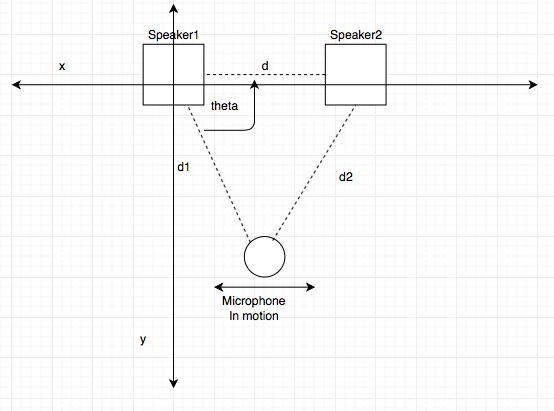
\includegraphics[width=9cm, height=9cm]{PCSetup}
\end{figure}

\subsection{Technical Details Sound Generation} \label{technical_details Sound Mixing}
In order to generate sounds MATLAB is used to generate 10 Sinusoidal waves, 5 for the left speaker and 5 for the right, each spaced 200 Hz apart. The process for generating the sounds can be seen in Algorithm 1.

\begin{algorithm}
\KwData{amp=1;}
\KwData{fs=80000;}
\KwData{duration=50;}
\KwData{values=0:1/fs:duration;}
\setlength{\parindent}{0cm}
\For { frequency from 18000 to 18800 }
{$wave\_left = wave\_left + amp*sin(2*pi*frequency*values);$
$frequency += 200;$}
\For { frequency from 19000 to 19800 }
{$wave\_right = wave\_right + amp*sin(2*pi*frequency*values);$
$frequency += 200;$}

$
combined = [wave\_left(:), wave\_right(:)];
$
$write(file, combined);$

\caption{How to generate Sinusoidal inaudible sounds}
\end{algorithm}

\subsection{Technical Details Receiver Design} \label{technical_details Receiver Design}
The receiver which processes the audio signals uses a continuous loop to run for some variable amount of time. Inside of the loop we take 44100 samples from the microphone and perform a Short Time Fourier Transform with 44100 points. This is also applies a Hamming window with 1764 points and an overlap of 50 percent. At this point the signal consists of all of the 10 frequencies transmitted from the speakers. We next perform maximal ratio combining by imposing the idea of a channel. We do this by imposing a window of 50 Hz around the center frequencies of each of the 10 frequencies we generated. Then for each channel we estimate the noise variance by taking the sum of all of the signals outside of where we expect the signal to fall and then averaging this value by the number of points used. We then weight each channel by the inverse of this value, which is a rough approximation of the inverse of the noise variance. Next the frequencies are split into two sets.  The weighted signals are then averaged with the other signals in their set and the the frequency exhibiting the strongest power is extracted from each set. We use these value to calculate the Doppler shift by finding the original frequency value it is closest to and taking the difference. If Doppler shift that is generated is greater than 10 Hz we throw this point out. In the event we throw the point out, we extract the maximum power signal in each channel and calculate the difference between each value and it's closest original frequency value. Then the Doppler shift calculation that is closest to the previous loops Doppler shift is selected as the Doppler shift. We specifically note that this technique of throwing out points in the event the Doppler shift is greater than 10 Hz may cause a biasing towards higher values for future calculations in the event no channel yields a Doppler shift estimate that is less than 10 Hz. Which is a potential source of error, however, the probability that this event will occur is somewhat small given the fact there are 10 frequency values.  The Doppler shift obtained is then used to estimate a distance between each of the speakers. Then given distance we estimate the angle between the speaker and the microphone and use that angle to then calculate an x y point. We also note that this point is the intersection of two concentric circles, each with their center at each of the speakers. This means there are potentially two intersections. However, for simplicity and because the second second intersection point tends to cause a larger distance jump from the microphone we do not calculate the second intersection point in the event one exists. 

\subsection{Setup-Android}
We used one Samsung SM-T320 tablet and two Logitech S-120 speakers for experiment 
hardware. The experiment setup is the same as the one mentioned above for our PC 
implementation. We keep the distance between the speaker to the device to be one meter
and the distance between two speakers also to be one meter. 

\subsection{Technical Details-Android}
The sampling rate we used is the same as the original paper, 44.1 KHz. It is also the 
default sampling rate supported by the device. By default, we uses 44,100 as the buffer
size to store the audio samples. Such size is chosen in order to provide the fine-grained
frequency resolution.
Because in Android system, there is no signal processing libraries to use, we cannot 
call STFT function in one line as we did in PC side. Thus the first issue is how to 
calculate frequency shift in Doppler shift. We used a third party FFT tool from 
\cite{FFT}. This FFT function will return the same number of points as the buffer size
of the stored signal. The even index of the FFT point are the imaginary part and the odd 
index of the FFT point are the real part. We then found the frequencies with the greatest
FFT value and subtracted it with the sending frequency to obtain the frequency shift. 
Then we are able to calculate the velocity. 

To improve the accuracy of the system, we also implement MRC in Android side, the 
technical detail is the same as above for the PC section. After applying MRC, the original
work uses Kalman filter to smooth the data. However, there is no such filter available in
Android system. Instead, we applied a third party filter from
\cite{SignalFilter} called OneEuroFilter to smooth the data.

After the post processing, we were able to get the frequency shift in each axis, averaging
five sound frequencies. Then we calculate the distance using the same equations mentioned
above.

\subsection{Lessons learned}
The knowledge we obtained from the project, specifically with the PC implementation in mind is we learned numerous pieces of signal processing theory, including why we would want to use a STFT as opposed to an FFT. We also learned tons about spacial and frequency diversity when we attempted to implement the maximal ratio combining portion of the project since most of the examples for diversity combining techniques center around spacial diversity as opposed to frequency diversity. Despite learning this, we still are yet to find a good example on Maximal Ratio Combining  for frequency diversity. Hence it is possible our implementation is theoretically flawed. We also learned how to implement the Kalman filter in MATLAB, which is not necessarily a simple task despite there being numerous resources on how to do it. Modeling the problem as a state transition function turns out to require even more knowledge of signal processing, beyond what even to this point we have obtained. Despite this we did make an attempt to figure out how to come up with a model for our problem, unfortunately more research is necessary to build the Kalman filtering into the code. One piece of the of the project which we did not attempt to implement was the particle filtering for estimation of the starting location of the microphone. This is our largest source of error by far and is the primary reason for regular bad results. We further hypothesize that we could obtain significantly better results for the project if we would have implemented this portion.
In Android side, The initial buffer size is chosen as 1759, which is the minimum
buffer size by default calculation using Android AudioRecorder class. 
Using buffer size of 1759 is no doubt too small for FFT. Such value
will lead to a very low frequency resolution, which will cause the distance calculation
to be very inaccurate. Same theory is also mentioned in the original work. The correct
buffer size should be 44100. However, this value did not work at the first place and 
it will lead the app to stop working immediately. One suspicious cause is the intensive
computing cost inside the while loop for the real time signal processing. Then we 
optimized the code to compute the maximum frequencies in linear time. This procedure 
allow the buffer size to be set as 44100. The app will run for approximate 15 seconds
before it crushes.
Even if the app will work for 15 seconds, this huge buffer size value will take one
second to record. A long FFT does not allow us to track the device in real time. In one
second, the device may move to other location. As a result, even though we were able to
obtain the fine grained frequency shift using our Android device, the tracking result 
may not be accurate due to the long FFT.

\section{EVALUATION} \label{evaluation}
The evaluation was carried out on both Android and PC platforms. To evaluate the PC platform we evaluate the general ability of the platform to trace given shapes since distance will always be inaccurate due to the lack of knowing where in global space the fact we did not implement the particle filter. If one were to use distance as a metric the implementation obtains a massive error calculation. Hence the need for a more qualitative evaluation. Additionally, we note that the platform only gives a window of around 8 to 10 seconds before error in all variables, x, y theta and velocity propagates to the point where the system becomes completely incorrect and neither tracks distance nor general shape.
%\end{document}  % This is where a 'short' article might terminate

%ACKNOWLEDGMENTS are optional
\subsection{Performance Analysis - Motion Tracking}
In figure 1 we can see the plot of tracing a simple straight line moving the microphone toward the speakers. We see the ground truth indicated by the + mark and the actual value of the microphone as *. Additionally, the time at which the point was obtained is included in the adjacent text, where t indicates the time at which the ground truth point would be obtained and ta represents the time at which the actual points are obtained. Additionally, due to a constant error of approximately 30 cm the graph takes this into account and normalizes the result by subtracting the error. From this image we see that a majority of the points near the beginning of the test are close to the ground truth values, however, as we see time approach the end of the test where $ta > 10$ we see very poor behavior from the system. This is most likely due to the error propagation.
\begin{figure}[h]
\caption{Tracing line in Y direction, while holding X constant}
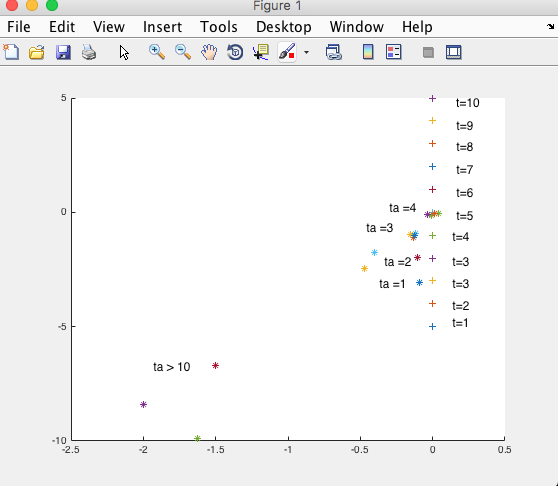
\includegraphics[width=9cm, height=11cm]{TracingY}
\end{figure}

\subsection{Inaudible Tone Frequency Choices}
Originally, we chose inaudible frequencies between 20kHz and 21.8 kHz. However, after attempting to use these frequencies it was observed that the power of the frequencies above 20kHz were very week. Due to this we switched to use the frequencies from 18kHz to 19.8kHz. The results of the PSD graphs can be seen in figures 4 and 5.

\begin{figure}[h]
\caption{PSD when using frequencies above 20kHz}
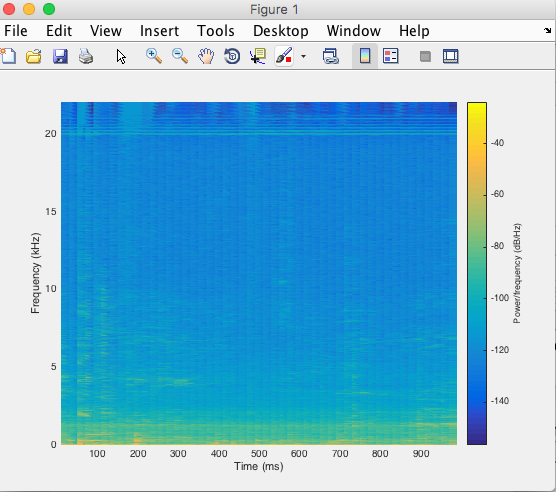
\includegraphics[width=9cm, height=11cm]{above20}
\end{figure}

\begin{figure}[h]
\caption{PSD when using frequencies above 18kHz to 19.8kHz}
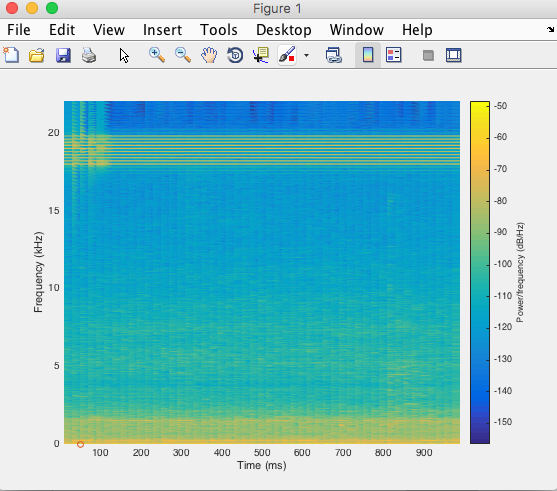
\includegraphics[width=9cm, height=11cm]{Below20}
\end{figure}

\subsection{Potential Improvements}
There are numerous potential improvements that could be made to the system in nearly every aspect. To start with a better implementation of Maximal Ratio Combining could be used, specifically one that does not discount the actual frequencies around the center of each channel for calculation of the noise variance. One other aspect for improvement is in the potential to further smooth the Doppler shift curve with Kalman Filtering; this however, would require much more research and evaluation in which transition function would best fit to the problem. Another improvement is answering the question of whether or not we actually need to calculate a global points in global space. One possible implementation could define both global and local coordinate spaces, where the local coordinate axis is with respect to the microphone and the global axis is with respect to the speakers. Then a method for deriving points in the global coordinate axis involves multiplying the result in the local coordinate axis by the transpose of the Jaobian. This idea comes from kinematics in robotic motion planning. Finally, one large issue we ran into when performing the evaluation is that the time to process the data in real time reached a point where the data that was being reported was old and mismatched in the timing. This is because the time it takes to complete one of the loops in the MATLAB program is approximately 1 second. The authors of the paper explicitly mention that 1 second is too long of a window in time for results to be accurate. One possible solution to this is to gather the data in a matrix in MATLAB for each instance of time and then calculate the x y pairs in a non-real time fashion. 
In Android side, we could use STFT packet instead of FFT to increase the accuracy
because a long FFT cannot track the device in real time. However, currently there is 
no STFT library available for Android platform. We could implement our own STFT. 
The original work applied STFT to use 1764 audio samples to still achieve 1 Hz frequency
resolution.

%
% The following two commands are all you need in the
% initial runs of your .tex file to
% produce the bibliography for the citations in your paper.
\bibliographystyle{abbrv}
\bibliography{sigproc}  % sigproc.bib is the name of the Bibliography in this case
% You must have a proper ".bib" file
%  and remember to run:
% latex bibtex latex latex
% to resolve all references
%
% ACM needs 'a single self-contained file'!
%
\end{document}